\section{Front-end}

	\subsection{Descrizione packages e classi}

	\subsubsection{SWEDesigner::Client}
		\begin{figure}[h!]
			\centering
			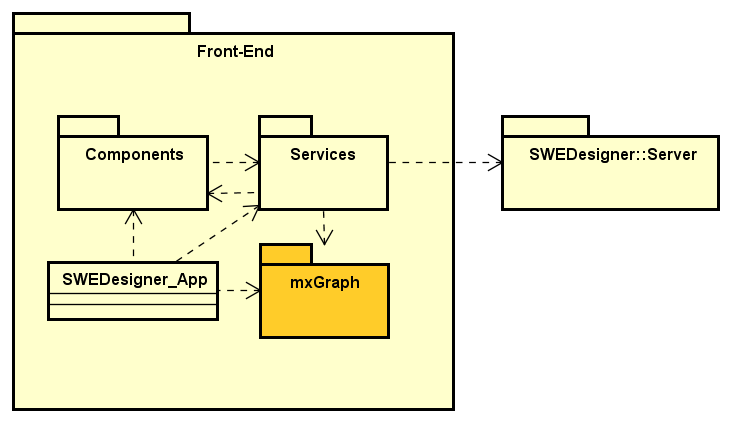
\includegraphics[scale=0.4]{Disegnetti/Front-End.png}
			\caption{Diagramma dei packages SWEDesigner::Client}
 		\end{figure}
		\begin{figure}
			\centering
			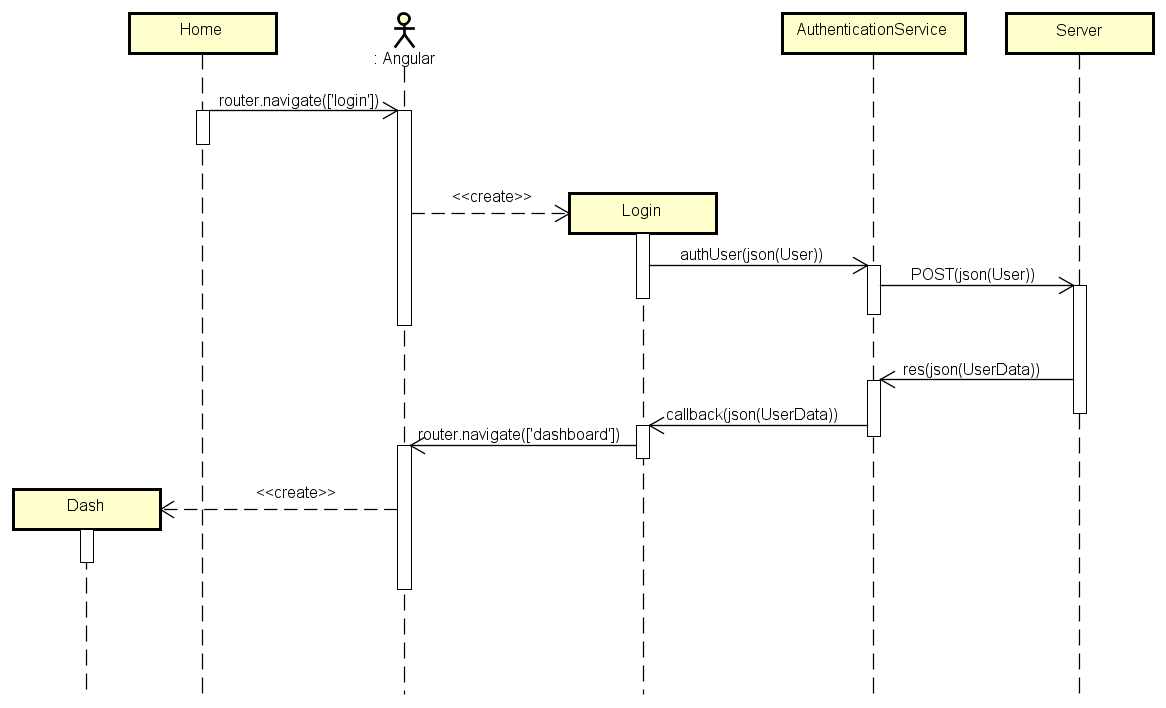
\includegraphics[scale=0.4]{Disegnetti/SequenceDiagram.png}
			\caption{Esempio di funzionamento dell'applicazione lato client}
		\end{figure}

		\paragraph{Informazioni sul Package}
		\begin{itemize}
			\item \textbf{Descrizione: }\\
			Package che racchiude tutta la componente di Front-end scritta in JavaScript.
			\item \textbf{Padre: }\\ SWEDesigner
			\item \textbf{Package contenuti: }
			\begin{itemize}
				\item SWEDesigner::Client::Components;
				\item SWEDesigner::Client::Services;
				\item SWEDesigner::Server;
			\end{itemize}
		\end{itemize}

		\paragraph{Informazioni sulle Classi}
		\begin{itemize}
			\item SWEDesigner::Client::SWEDesignerApp
			\begin{itemize}
				\item \textbf{Descrizione: }\\
				Questa classe detta anche \emph{root module} si occupa di definire i
				moduli che compongono l'applicazione e come istanziarli.
				\item \textbf{Utilizzo: }\\
				È il primo modulo su cuo viene fatto il bootstrap per lanciare l'applicazione
			\end{itemize}
		\end{itemize}


		\subsubsection{SWEDesigner::Client::Components}
		 \begin{figure}[h!]
		\centering
		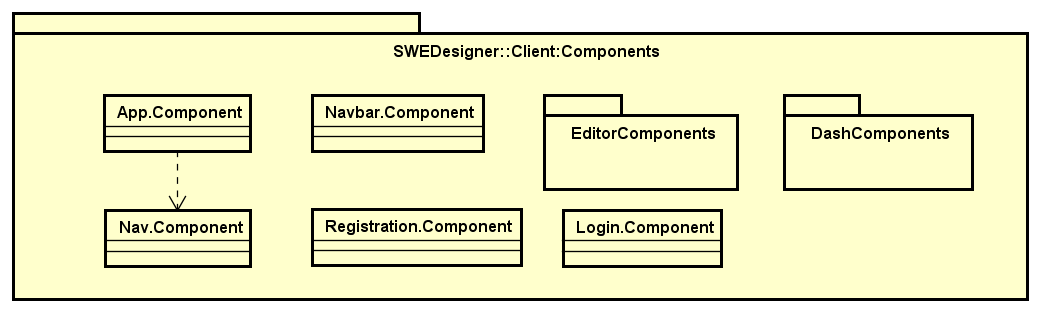
\includegraphics[scale=0.4]{Disegnetti/SWEDesigner__Client_Components.png}
		\caption{Diagramma dei packages SWEDesigner::Client::Components}
 		\end{figure}
		\paragraph{Informazioni sul Package}
		\begin{itemize}
			\item \textbf{Descrizione: }\\
			Questo package contiene tutti i components dell'applicazione
			\item \textbf{Padre: }\\ SWEDesigner::Client
			\item \textbf{Package contenuti: }
			\begin{itemize}
				\item SWEDesigner::Client::Components::EditorComponents;
				\item SWEDesigner::Client::Components::DashComponents;
			\end{itemize}
		\end{itemize}

		\paragraph{Informazioni sulle Classi}
		\begin{itemize}
			\item SWEDesigner::Client::Components::AppComponent
			\begin{itemize}
				\item \textbf{Descrizione: }\\
				Il component descrive un contenitore per la barra di navigazione e le altre
				componenti dell'applicazione le quali sono istanziate dinamicamente all'
				interno del template http;
				\item \textbf{Utilizzo: }\\
				AppComponent è il primo component che viene istanziato tramite bootsrap.
			\end{itemize}
			\item SWEDesigner::Client::Components::NavbarComponent
			\begin{itemize}
				\item \textbf{Descrizione: }\\
				Questo component permette la navigazione all'interno dell'applicazione
				tramite links;
				\item \textbf{Utilizzo: }\\
				NavbarComponent è istanziato per bootstrap subito dopo dell'AppComponent
			\end{itemize}
			\item SWEDesigner::Client::Components::RegistrationComponent
			\begin{itemize}
				\item \textbf{Descrizione: }\\
				È il componente che descrive la pagina di registrazione dell'applicazione,
				mette a disposizione dell'utente un form dove iserire le informazioni
				necessarie alla creazione di un nuovo account utente. Gestisce le
				operazioni e la logica applicativa per la registrazione servendosi dei
				metodi forniti dal servizio AuthenticationService;
				\item \textbf{Utilizzo: }\\
				Questo componente viene instanziato dinamicamente dal servizio Router del
				 framework Angular qunado viene richiesta la pagina di registrazione.
			\end{itemize}
			\item SWEDesigner::Client::Components::LoginComponent
			\begin{itemize}
				\item \textbf{Descrizione: }\\
				È il componente che descrive la pagina di login dell'applicazione,
				mette a disposizione dell'utente un form dove iserire username e password.
				Gestisce le operazioni e la logica applicativa per il login servendosi dei
				metodi forniti dal servizio AuthenticationService;
				\item \textbf{Utilizzo: }\\
				Questo componente viene instanziato dinamicamente dal servizio Router del
				framework Angular qunado viene richiesta la pagina di login.
			\end{itemize}
		\end{itemize}

		\subsubsection{SWEDesigner::Client::Components::EditorComponents}
		 \begin{figure}[h!]
		\centering
		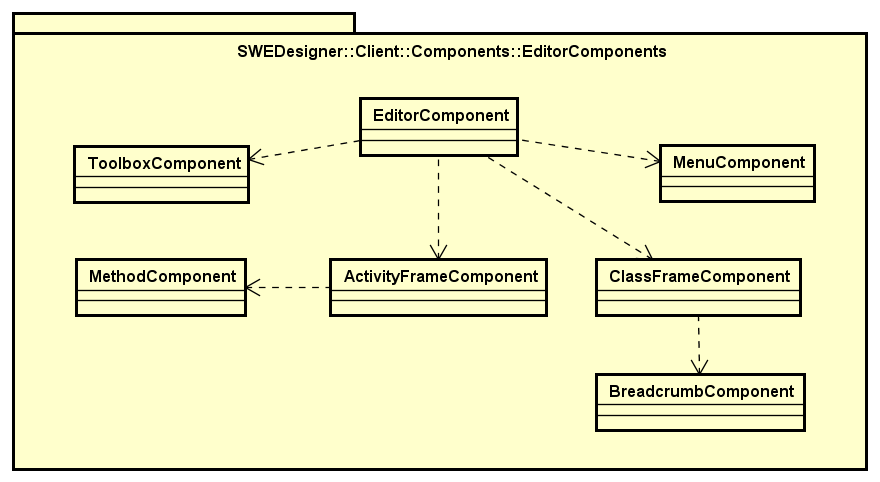
\includegraphics[scale=0.4]{Disegnetti/SWEDesigner__Client__Components__EditorComponents.png}
		\caption{Diagramma dei packages SWEDesigner::Client::Components::EditorComponents}
 		\end{figure}
		\paragraph{Informazioni sul Package}
		\begin{itemize}
			\item \textbf{Descrizione: }\\
			Il package contiene tutte le components riguardanti l'editor dei diagrammi.
			\item \textbf{Padre: }\\ SWEDesigner::Client::Components
		\end{itemize}

		\paragraph{Informazioni sulle Classi}
		\begin{itemize}
			\item SWEDesigner::Client::Components::EditorComponents::ToolboxComponent
			\begin{itemize}
				\item \textbf{Descrizione: }\\
				ToolboxComponent descrive il menu dal quale l'utente può selezionare gli
				strumenti per disegnare i diagrammi all'interno degli appositi frame. Si
				occupa delle operazioni e della parte logica, riguardante la costruzione
				dei diagrammi, servendosi dei metodi forniti dal servizio ProjManagService e
				della API della libreria grafica;
				\item \textbf{Utilizzo: }\\
				MenuComponent componente viene istanziato per bootstrap dopo che è stato
				istanziato il component EditorComponent.
			\end{itemize}
			\item SWEDesigner::Client::Components::EditorComponents::EditorComponent
			\begin{itemize}
				\item \textbf{Descrizione: }\\
				Component che definisce la pagina dell'editor di diagrammi, contiene all'interno
				del template html gli attributi ToolboxComponent, MenuComponent,
				ClassFrameComponent, ActivityFrameComponent;
				\item \textbf{Utilizzo: }\\
				Questo componente viene instanziato dinamicamente dal servizio Router del
				framework Angular quando viene richiesta la pagina dell'editor diagrammi.
			\end{itemize}
			\item SWEDesigner::Client::Components::EditorComponents::MenuComponent
			\begin{itemize}
				\item \textbf{Descrizione: }\\
				Component che descrive il menu dell'edito dei diagrammi. Il menu da la
				possibilità all'utente di salvare, esportare, compilare o uscire dal progetto
				visualizzato nell'editor dei diagrammi. Si occupa delle operazioni e della
				logica applicativa per le operazioni, precedentemente elencate, servendosi
				dei metodi messi a disposizione dai servizi contenuti nel package
				ProjectServices;
				\item \textbf{Utilizzo: }\\
				MenuComponent componente viene istanziato per bootstrap dopo che è stato
				istanziato il component EditorComponent.
			\end{itemize}
			\item SWEDesigner::Client::Components::EditorComponents::MethodComponent
			\begin{itemize}
				\item \textbf{Descrizione: }\\
				MethodComponent descrive il frame dove l'utente può disegnare gli activity
				diagrams per definire i metodi di una classe disegnata nel frame del
				diagramma delle classi. Si occupa delle operazioni e logica applicativa per
				la generazione dei diagrammi dei metodi, par fare questo si serve dell'API
				della libreria grafica;
				\item \textbf{Utilizzo: }\\
				Questo component viene istaziato per bootstrap dopo l'istanziazione del
				componente ClassFrameComponent.
			\end{itemize}
			\item SWEDesigner::Client::Components::EditorComponents::ActivityFrameComponent
			\begin{itemize}
				\item \textbf{Descrizione: }\\
				Component che descrive la struttura del frame dove l'utente può visualizzare
				l'activity frame che rappresenta il flusso logico del programma. Si occupa
				delle operazioni che portano alla corretta visualizzazione del diagramma
				servendosi dell'API della libreria grafica;
				\item \textbf{Utilizzo: }\\
				Questo component viene istanziato per bootstrap dopo l'istanziazione
				del component EditorComponent.
			\end{itemize}
			\item SWEDesigner::Client::Components::EditorComponents::ClassFrameComponent
			\begin{itemize}
				\item \textbf{Descrizione: }\\
				ClassFrameComponent descrive la struttura del frame dove l'utente può
				generare, modificare e cancellare le classi che compongono il suo progetto.
				Si occupa delle operazioni che portano alla corretta visualizzazione del diagramma
				servendosi dell'API della libreria grafica;
				\item \textbf{Utilizzo: }\\
				Questo component viene istanziato per bootstrap dopo l'istanziazione
				del component EditorComponent.
			\end{itemize}
			\item SWEDesigner::Client::Components::EditorComponents::BreadcrumbComponent
			\begin{itemize}
				\item \textbf{Descrizione: }\\
				Component che facilita la navigazione all'interno del ActivityFrameComponent;
				\item \textbf{Utilizzo: }\\
				BreadcrumbComponent component viene istanziato per bootstrap dopo l'istanziazione
				del component ActivityFrameComponent.
			\end{itemize}
		\end{itemize}

		\subsubsection{SWEDesigner::Client::Components::DashboardComponents}
		 \begin{figure}[h!]
		\centering
		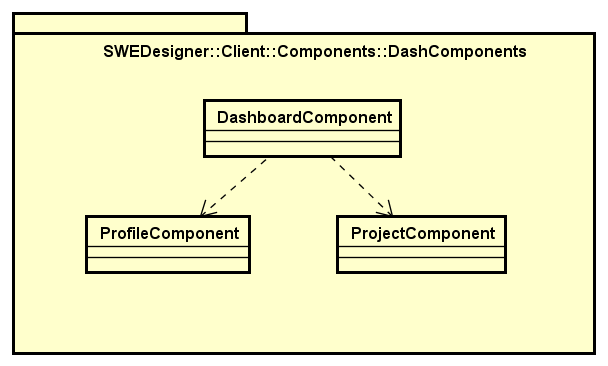
\includegraphics[scale=0.4]{Disegnetti/SWEDesigner__Client__Components__DashComponents.png}
		\caption{Diagramma dei packages SWEDesigner::Client::Components::DashComponents}
 		\end{figure}
		\paragraph{Informazioni sul Package}
		\begin{itemize}
			\item \textbf{Descrizione: }\\
			Il package contiene tutti i components riguardanti la gestione del profilo
			e dei progetti dell'utente.
			\item \textbf{Padre: }\\ SWEDesigner::Client::Components
		\end{itemize}

		\paragraph{Informazioni sulle Classi}
		\begin{itemize}
			\item SWEDesigner::Client::Components::DashComponents::DashComponent
			\begin{itemize}
				\item \textbf{Descrizione: }\\
				Component che definisce la pagina dove l'utente è reindirizzato dopo aver
				effettuato il login, contiene all'interno del template html gli elementi
				per l'istanziazione del ProfileComponent e del ProjectComponent.
				\item \textbf{Utilizzo: }\\
				Questo componente viene instanziato dinamicamente dal servizio Router del
				framework Angular subito dopo aver effettuato il login.
			\end{itemize}
			\item SWEDesigner::Client::Components::DashComponents::ProfileComponent
			\begin{itemize}
				\item \textbf{Descrizione: }\\
				ProfileComponent contiene le informazioni personali dell'utente. Si occupa
				delle operazioni che permettono il recupero dei dati utente servendosi di
				metodi forniti dal servizio AuthenticationService.
				\item \textbf{Utilizzo: }\\
				Questo componenet viene istanziato per bootstrap dopo l'istanziazione
				del component DashComponent.
			\end{itemize}
			\item SWEDesigner::Client::Components::DashComponents::ProjectComponent
			\begin{itemize}
				\item \textbf{Descrizione: }\\
				ProfileComponent contiene la lista dei progetti salvati dall'utente, e
				fornisce dei metodi per la modifica e la cancellazione dei progetti. Si
				occupa delle operazioni che permettono il recupero delle informazioni sui
				progetti servendosi di metodi forniti dal servizio ProjManagService.
				\item \textbf{Utilizzo: }\\
				Questo componenet viene istanziato per bootstrap dopo l'istanziazione
				del component DashComponent.
			\end{itemize}
		\end{itemize}

\subsubsection{SWEDesigner::Client::Service}
		 \begin{figure}[h!]
		\centering
		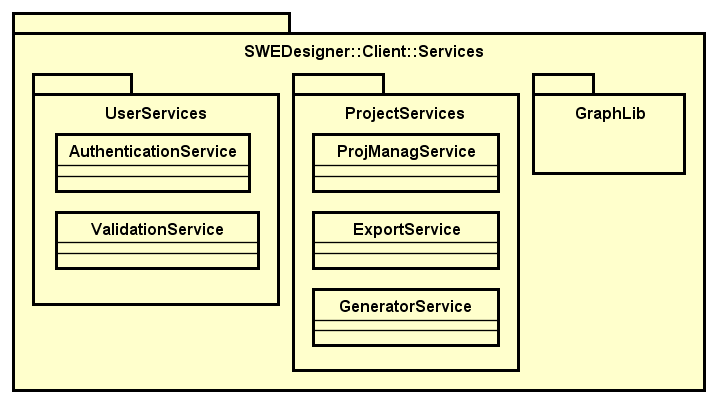
\includegraphics[scale=0.4]{Disegnetti/SWEDesigner__Client__Services.png}
		\caption{Diagramma dei packages SWEDesigner::Client::Service}
 		\end{figure}
		\paragraph{Informazioni sul Package}
		\begin{itemize}
			\item \textbf{Descrizione: }\\
			Il package contiene i servizi per le operazioni con la libreria grafica
			\emph{jointJS} e con il server.
			\item \textbf{Padre: }\\ SWEDesigner::Client
			\item \textbf{Package contenuti: }
			\begin{itemize}
				\item SWEDesigner::Client::Services::UserServices;
				\item SWEDesigner::Client::Services::ProjectServices;
				\item SWEDesigner::Client::Services::GraphLib;
			\end{itemize}
		\end{itemize}

	\subsubsection{SWEDesigner::Client::Services::UserServices}
		\paragraph{Informazioni sul Package}
		\begin{itemize}
			\item \textbf{Descrizione: }\\
			Questo package contiene le classi che offrono servizi di registrazione, login
			e recupero dati utente dal server.
			\item \textbf{Padre: }\\ SWEDesigner::Client::Services
		\end{itemize}

		\paragraph{Informazioni sulle Classi}
		\begin{itemize}
			\item SWEDesigner::Client::Services::UserServices::AuthenticationService
			\begin{itemize}
				\item \textbf{Descrizione: }\\
				Questa classe definisce i metodi di comunicazione con il server per quanto
				riguarda i servizi di registrazione, login e recupero dati utente;
				\item \textbf{Utilizzo: }\\
				La classe è istanziata dal framework Angular e i suoi metodi sono utilizzati
				dai components LoginComponent, RegistrationComponent e ProfileComponent.
			\end{itemize}
			\item SWEDesigner::Client::Services::UserServices::ValidationService
			\begin{itemize}
				\item \textbf{Descrizione: }\\
				ValidationService descrive dei metodi per verificare la validità degli input
				operati dall'utente;
				\item \textbf{Utilizzo: }\\
				Essa è istanziata dal framework Angular e i suoi metodi sono utilizzati
				dal component RegistrationComponent.
			\end{itemize}
		\end{itemize}


		\subsubsection{SWEDesigner::Client::Services::ProjectServices}
		\paragraph{Informazioni sul Package}
		\begin{itemize}
			\item \textbf{Descrizione: }\\
			Questo package contiene i servizi inerenti alla gestione dei progetti e
			l'operatività dell'editor.
			\item \textbf{Padre: }\\ SWEDesigner::Client::Services
		\end{itemize}

		\paragraph{Informazioni sulle Classi}
		\begin{itemize}
			\item SWEDesigner::Client::Services::ProjectServices::ProjManagService
			\begin{itemize}
				\item \textbf{Descrizione: }\\
				Classe che definisce le operazioni inerenti alla gestione dei progetti
				dell'utente;
				\item \textbf{Utilizzo: }\\
				ProjManagService è istanziata da Angular, i suoi metodi venogo utilizzati
				dai components ProjectComponent e MenuComponent.
			\end{itemize}
			\item SWEDesigner::Client::Services::ProjectServices::ExportService
			\begin{itemize}
				\item \textbf{Descrizione: }\\
				ExportServices definisce le operazioni necessarie a esportare il progetto
				dell'utente;
				\item \textbf{Utilizzo: }\\
				Essa è istaziata dal framework Angular e i suoi metodi sono utilizzati
				dal component MenuComponent.
			\end{itemize}
			\item SWEDesigner::Client::Services::ProjectServices::GeneratorService
			\begin{itemize}
				\item \textbf{Descrizione: }\\
				Classe che definisce le operazioni necessarie alla compilazione del
				progetto dell'utente;
				\item \textbf{Utilizzo: }\\
				GeneratorService è istanziata dal framework Angular e utilizzata dal
				components MenuComponet.
			\end{itemize}
		\end{itemize}
